%%
%% This is file `sample-sigconf.tex',
%% generated with the docstrip utility.
%%
%% The original source files were:
%%
%% samples.dtx  (with options: `sigconf')
%% 
%% IMPORTANT NOTICE:
%% 
%% For the copyright see the source file.
%% 
%% Any modified versions of this file must be renamed
%% with new filenames distinct from sample-sigconf.tex.
%% 
%% For distribution of the original source see the terms
%% for copying and modification in the file samples.dtx.
%% 
%% This generated file may be distributed as long as the
%% original source files, as listed above, are part of the
%% same distribution. (The sources need not necessarily be
%% in the same archive or directory.)
%%
%% Commands for TeXCount
%TC:macro \cite [option:text,text]
%TC:macro \citep [option:text,text]
%TC:macro \citet [option:text,text]
%TC:envir table 0 1
%TC:envir table* 0 1
%TC:envir tabular [ignore] word
%TC:envir displaymath 0 word
%TC:envir math 0 word
%TC:envir comment 0 0
%%
%%
%% The first command in your LaTeX source must be the \documentclass command.
\documentclass[sigconf]{acmart}
%% NOTE that a single column version may be required for 
%% submission and peer review. This can be done by changing
%% the \doucmentclass[...]{acmart} in this template to 
%% \documentclass[manuscript,screen]{acmart}
%% 
%% To ensure 100% compatibility, please check the white list of
%% approved LaTeX packages to be used with the Master Article Template at
%% https://www.acm.org/publications/taps/whitelist-of-latex-packages 
%% before creating your document. The white list page provides 
%% information on how to submit additional LaTeX packages for 
%% review and adoption.
%% Fonts used in the template cannot be substituted; margin 
%% adjustments are not allowed.
%%
%%
%% \BibTeX command to typeset BibTeX logo in the docs
\AtBeginDocument{%
  \providecommand\BibTeX{{%
    \normalfont B\kern-0.5em{\scshape i\kern-0.25em b}\kern-0.8em\TeX}}}

%% Rights management information.  This information is sent to you
%% when you complete the rights form.  These commands have SAMPLE
%% values in them; it is your responsibility as an author to replace
%% the commands and values with those provided to you when you
%% complete the rights form.
\setcopyright{acmcopyright}
\copyrightyear{2023}
\acmYear{2023}
\acmDOI{} %% isto

%% These commands are for a PROCEEDINGS abstract or paper.
\acmConference[G53]{PRI}{October-09, 2023}{Porto, Portugal}
%
%  Uncomment \acmBooktitle if th title of the proceedings is different
%  from ``Proceedings of ...''!
%
%\acmBooktitle{Woodstock '18: ACM Symposium on Neural Gaze Detection,
%  June 03--05, 2018, Woodstock, NY} 
\acmPrice{15.00}
\acmISBN{978-1-4503-XXXX-X/18/06}


%%
%% Submission ID.
%% Use this when submitting an article to a sponsored event. You'll
%% receive a unique submission ID from the organizers
%% of the event, and this ID should be used as the parameter to this command.
%%\acmSubmissionID{123-A56-BU3}

%%
%% For managing citations, it is recommended to use bibliography
%% files in BibTeX format.
%%
%% You can then either use BibTeX with the ACM-Reference-Format style,
%% or BibLaTeX with the acmnumeric or acmauthoryear sytles, that include
%% support for advanced citation of software artefact from the
%% biblatex-software package, also separately available on CTAN.
%%
%% Look at the sample-*-biblatex.tex files for templates showcasing
%% the biblatex styles.
%%

%%
%% The majority of ACM publications use numbered citations and
%% references.  The command \citestyle{authoryear} switches to the
%% "author year" style.
%%
%% If you are preparing content for an event
%% sponsored by ACM SIGGRAPH, you must use the "author year" style of
%% citations and references.
%% Uncommenting
%% the next command will enable that style.
%%\citestyle{acmauthoryear}

%%
%% end of the preamble, start of the body of the document source.
\begin{document}

%%
%% The "title" command has an optional parameter,
%% allowing the author to define a "short title" to be used in page headers.
\title{Privago: Hotels Search System}

%%
%% The "author" command and its associated commands are used to define
%% the authors and their affiliations.
%% Of note is the shared affiliation of the first two authors, and the
%% "authornote" and "authornotemark" commands
%% used to denote shared contribution to the research.
\author{André Costa}
\email{up201905916@edu.fe.up.pt}
\affiliation{%
  \institution{Faculty of Engineering - University of Porto}
  \city{Porto}
  \country{Portugal}
}

\author{André Ávila}
\email{up202006767@edu.fe.up.pt}
\affiliation{%
  \institution{Faculty of Engineering - University of Porto}
  \city{Porto}
  \country{Portugal}
}

\author{Fábio Sá}
\email{up202007658@edu.fe.up.pt}
\affiliation{%
  \institution{Faculty of Engineering - University of Porto}
  \city{Porto}
  \country{Portugal}
}

\author{Fábio Morais}
\email{up202008052@edu.fe.up.pt}
\affiliation{%
  \institution{Faculty of Engineering - University of Porto}
  \city{Porto}
  \country{Portugal}
}


%%
%% The abstract is a short summary of the work to be presented in the
%% article.
\begin{abstract}
  The internet's exponential growth demands appropriate systems for harnessing and connecting this massive information resource. This project addresses this need by focusing on the hotel industry, where reviews play a crucial role in shaping consumer choices. This article aims to provide a clear and well-documented explanation of the work needed in developing a robust search engine for hotel reviews. To accomplish this, data is collected from multiple sources, cleaned and prepared, and in-depth data analysis is undertaken.
\end{abstract}

%%
%% The code below is generated by the tool at http://dl.acm.org/ccs.cfm.
%% Please copy and paste the code instead of the example below.
%%
\begin{CCSXML}
<ccs2012>
<concept>
<concept_id>10002951.10003317.10003325</concept_id>
<concept_desc>Information systems~Information retrieval query processing</concept_desc>
<concept_significance>100</concept_significance>
</concept>
</ccs2012>
\end{CCSXML}

\ccsdesc[100]{Information systems~Information retrieval query processing}


%%
%% Keywords. The author(s) should pick words that accurately describe
%% the work being presented. Separate the keywords with commas.
\keywords{Hotels, Reviews, Information, Dataset, Data Retrieval, Data Preparation, Data Analysis, Data Processing, Data Refinement, Pipeline, Data Domain Conceptual Model
}

%% A "teaser" image appears between the author and affiliation
%% information and the body of the document, and typically spans the
%% page.
\begin{teaserfigure}
  \includegraphics[width=\textwidth]{imgs/teaser.jpg}
  \caption{Hotel}
  \label{fig:teaser}
\end{teaserfigure}


%%
%% This command processes the author and affiliation and title
%% information and builds the first part of the formatted document.
\maketitle

\section{Introduction}
This paper is developed as part of the course "Information Processing and Retrieval" (PRI) within the first year of the Master's in Informatics and Computing Engineering (MEIC) at the Faculty of Engineering of the University of Porto (FEUP).

The choice of the hotel reviews theme is motivated by its significant relevance and the rich diversity of attributes it encompasses. Hotel reviews, as a research focus, hold substantial importance in the modern information landscape. They not only provide valuable insights into the hospitality industry but also serve as a prime example of data diversity, combining numerical rates, submission dates, and personal, subjective narratives. This diversity introduces intricacies in data structuring and presents challenges in contextual search, making it an ideal choice for aligning the search system with real-world scenarios. Thus, this theme strongly resonates with the course objectives, emphasizing practical applicability and the development of robust information retrieval solutions.

This document is structured into several major sections, each tailored to fulfill the objectives of Milestone 1. We commence with \textbf{Data Extraction and Enrichment}, where we introduce the data sources, briefly characterize the datasets, and assess data quality. Subsequently, \textbf{Data Preparation} outlines the selection criteria, processing methods, and data storage procedures for hotel-related information and associated reviews, following a clear and reproducible pipeline.

In \textbf{Data Characterization} we delve into the evaluation and visualization of the refined data. This involves examining various criteria and relationships, from the Domain Conceptual Model to Word Clouds. Finally, \textbf{Possible Search Tasks} and \textbf{Conclusions and Future Work} provide an overarching interpretation of the results, guiding the identification of suitable research objectives for the project's next phase.

\section{Data Extraction and Enrichment}

After conducting research for relevant data in terms of variety and quantity, four datasets from different regions were selected through the Kaggle platform \cite{kaggle}. Table ~\ref{tab:initFreq} provides a characterization of the acquired datasets:

\begin{table}[h]
\small
\caption{Initial datasets characterization}
\label{tab:initFreq}
\begin{tabular}{lllll}
\toprule
Dataset & Features & Hotels & Reviews & Size(MBs)\\
\midrule
Datafiniti's Hotel Reviews & 26 & 1400 & 10000 & 124.45 \\
Hotel Review Insights & 7 & 570 & 7000 & 1.31 \\
London Hotel Reviews & 6 & 20 & 27329 & 22.85 \\
Europe Hotel Reviews & 17 & 1493 & 515000 & 238.15 \\
\bottomrule
\end{tabular}
\end{table}


The Datafiniti's Hotel Reviews \cite{Datafiniti's_Hotel_Reviews} dataset was taken from Datafiniti's Business Database \cite{Datafiniti's_Business_Database} through sampling. Hotel Review Insights \cite{Hotel_Review_Insights} is a compilation of hotels around the world through web-scraping of reviews found on Booking.com \cite{Booking}. London Hotel Reviews \cite{London_Hotel_Reviews} is a sample taken and partially refined from a DataStock dataset \cite{DataStock}. Finally, Europe Hotel Reviews \cite{Europe_Hotel_Reviews} also results from web scrapping of hotel reviews across Europe published on Booking.com \cite{Booking}.

All datasets have a public use license and, according to the Kaggle platform, a usability index greater than 8. This index is justified, given that the elimination of null, repeated or non-informative entries practically did not eliminate nothing.

The datasets contain common features, numerical data, such as rate, review date, and textual data, such as review text, hotel location and name. The last dataset contains two additional parameters, positive review and negative review. The features stated were extracted in this step and refined in Data Preparation.


\section{Data Preparation}

In this section, is presented the structured data preparation pipeline that was developed for the project. This pipeline embrace various data cleaning and restructuring procedures aimed at achieving a clean, uniform, and ready to analyze dataset. The goal of this stage is to build a strong basis for insightful analysis.

The data preparation process began with a comprehensive cleaning phase, where the primarly focus was the removal of records containing \textbf{empty or null values} in any attribute. Simultaneously, was identified and eliminated incomplete or uninformative data, including strings with \textbf{uninformative text}, such as "no comments available for this review.", using Python. This combined cleaning step ensured that the dataset was cleansed in detail for the normalization phase.

With the data cleaned, attention was turned to \textbf{attribute normalization}. Given the presence of diverse datasets with varying formats, comprehensive normalization process was needed. This included standardizing attributes such as \textbf{"positive\_reviews"} and \textbf{"negative\_reviews"} into a unified \textbf{"review\_text"} attribute for the 4th dataset as is demonstrated in the Pipeline Diagram [Figure \ref{fig:pipeline}]. Additionally, \textbf{date formats} were normalized to ensure uniformity and suitability for analysis. The date format was set as "year-month" due to the absence of day-specific review information in the second dataset and its irrelevance to the research targets. In fact, people search for seasons of the year, months, and not for a specific day. \textbf{Rate scales} were also normalized to a common range and converted to floating-point values, facilitating comparative analysis ([0.0, 5.0]).

In addiction, was established a \textbf{standardized naming} convention to address variations in \textbf{hotel names}, such as from \textit{"45 Park Lane - Dorchester Collection"} to \textit{"45 Park Lane Dorchester Collection"}. This step was necessary to facilitate the aggregation step and the addition of the feature "average\_rate" to each hotel entity, referenced below. \textbf{Location standardization} involved reducing location names to their last two words, preserving only the capital and country names.

To gain insights into the textual content, we calculated the temporary column \textbf{word count} for each review across all datasets. This analysis was facilitated using the Pandas \cite{Pandas} Python tool, allowing us to extract valuable information such as quartile ranges and make informed decisions during the review deletion phase. This process enabled us to identify and manage reviews with either an insufficient word count or an excessively high word count. We achieved this by removing reviews falling below the 25\% threshold (first quartile) and those exceeding the 75\% threshold (fourth quartile). This step was done separately for each dataset, due to the discrepation of each average word counting [Figure \ref{fig:reviewWords1}] [Figure \ref{fig:reviewWords3}].

At this stage, all the datasets were successfully merged into a single, consolidated dataset, which streamlined the remaining preparation tasks. These tasks commenced with the computation of the temporary column \textbf{"average\_rate"} for each unique hotel. This information may prove valuable for defining search criteria in future milestones.

After completing the aforementioned steps, the next phase involved determining the minimum and maximum number of \textbf{reviews per hotel} to be retained. To accomplish this, the same approach used for analyzing the number of words per review was employed, utilizing the Pandas \cite{Pandas} .describe() function. This statistical analysis provided essential insights into the distribution of reviews across hotels.

First, hotels with fewer reviews, falling below the established minimum threshold (first quartile), were addressed, and they were subsequently removed from the dataset. This step was crucial in ensuring that the dataset focused exclusively on hotels with a substantial volume of reviews, thus providing more meaningful insights.

Subsequently, hotels with an excessive number of reviews were taken into account. To handle this situation, a strategy was implemented, allowing the selection and retention of reviews while preserving the proportion of reviews per rate category for each specific hotel, i.e., its global rate. This approach guaranteed a balance between the "average\_rate" and the rate of the selected reviews.

The final step in the data preparation phase involved organizing the data into the \textbf{desired JSON file format}, which was designed based on our UML diagram [Figure \ref{fig:monthsDistribution}] and with a focus on the primary objective of the search tool. This format consisted of a collection of JSON objects, each representing a "Hotel" entity. Within each "Hotel" object, were included not only its associated attributes (name, location, average\_rate) but also the related reviews, presented as JSON objects themselves. Each review has a corresponding text, rate and submission date.

\begin{figure}[h]
  \centering
  \includegraphics[width=\linewidth]{imgs/pipeline.png}
  \caption{Data preparation pipeline}
  \Description{The figure shows a diagram that starts with the four data sources as csv files}
  \label{fig:pipeline}
\end{figure}

\section{Data Characterization}

In this section there is a characterization of the documents that are produced by the pipeline. The graphs and tables were obtained using the Matplotlib \cite{Matplotlib}, Numpy \cite{Numpy} and NLTK \cite{NLTK} libraries.

\subsection{Reviews Word Cloud}

\begin{figure}[H]
  \centering
  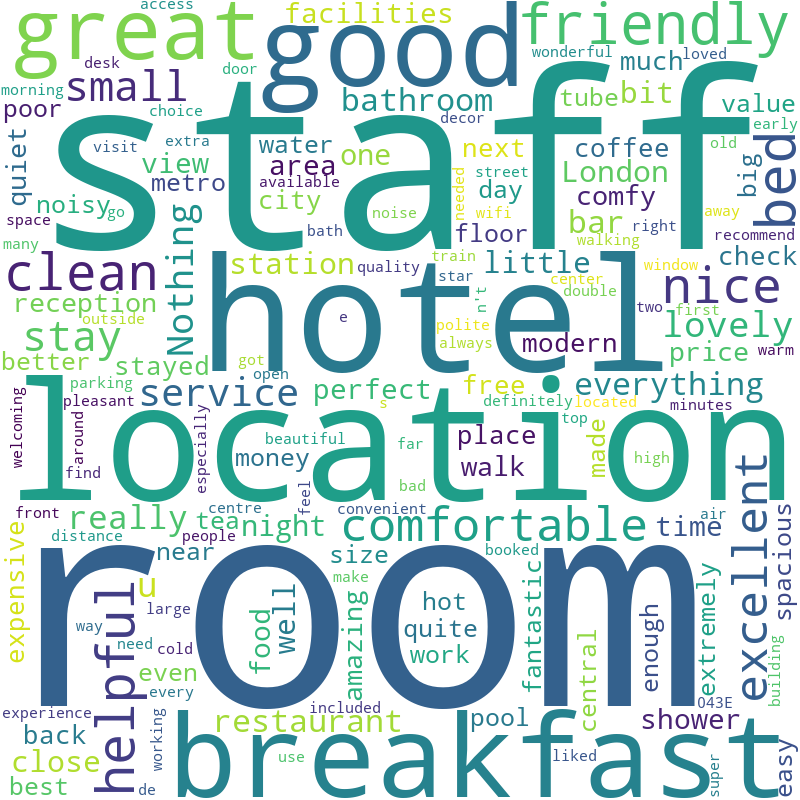
\includegraphics[width=\linewidth]{imgs/reviews_wordcloud.png}
  \caption{Reviews Word Cloud}
  \Description{TODO}
  \label{fig:wordcloud}
\end{figure}

The word cloud based on the texts of the reviews supports the search tasks of the next milestone as well as the contextual search to be implemented. As expected, the words that stand out the most are those intrinsically related to the hotel industry, such as "staff", "room", "location", "breakfast". Generally, the highlighted words have a neutral tone, although several with a very positive connotation are also detectable, such as "clean", "great", "lovely", "excellent", which can also be proven by the average rate [Figure \ref{fig:averageRateDistribution}] given to hotels.

\subsection{Hotel location distribution}

Figure \ref{fig:hotelLocationDistribution} shows the distribution of the 10 most frequent hotel locations in the system. As expected, the capitals and large cities of the main tourism countries concentrate the largest number of hotels and their reviews.

\subsection{Average rate distribution}

As we can see in figure \ref{fig:averageRateDistribution} Hotels tend to have very good reviews. The result is encouraged by their locations, as the majority are in cities with major tourist attractions and therefore with a greater cadence of reviews.

\subsection{Reviews per year}

From the analysis of the figure \ref{fig:reviewsDistributionYear}, it can be concluded that the system includes hotels with reviews from 2010 to 2023. However, the choice of initial datasets with information relating mainly to the period 2015 and 2017 influenced their representativeness.

Let's look, for example, at the distribution of reviews by month in 2016 in the figure \ref{fig:monthsDistribution}:

In fact, it is December when the number of reviews is higher, losing prominence after the start of the new year. This period corresponds to the time when people normally take vacations and therefore choose to travel. This pattern is repeated for the other years under analysis.

\subsection{Data Conceptual Model}

After the Data preparation phase, our documents contain the following relationships:

\begin{figure}[H]
  \centering
  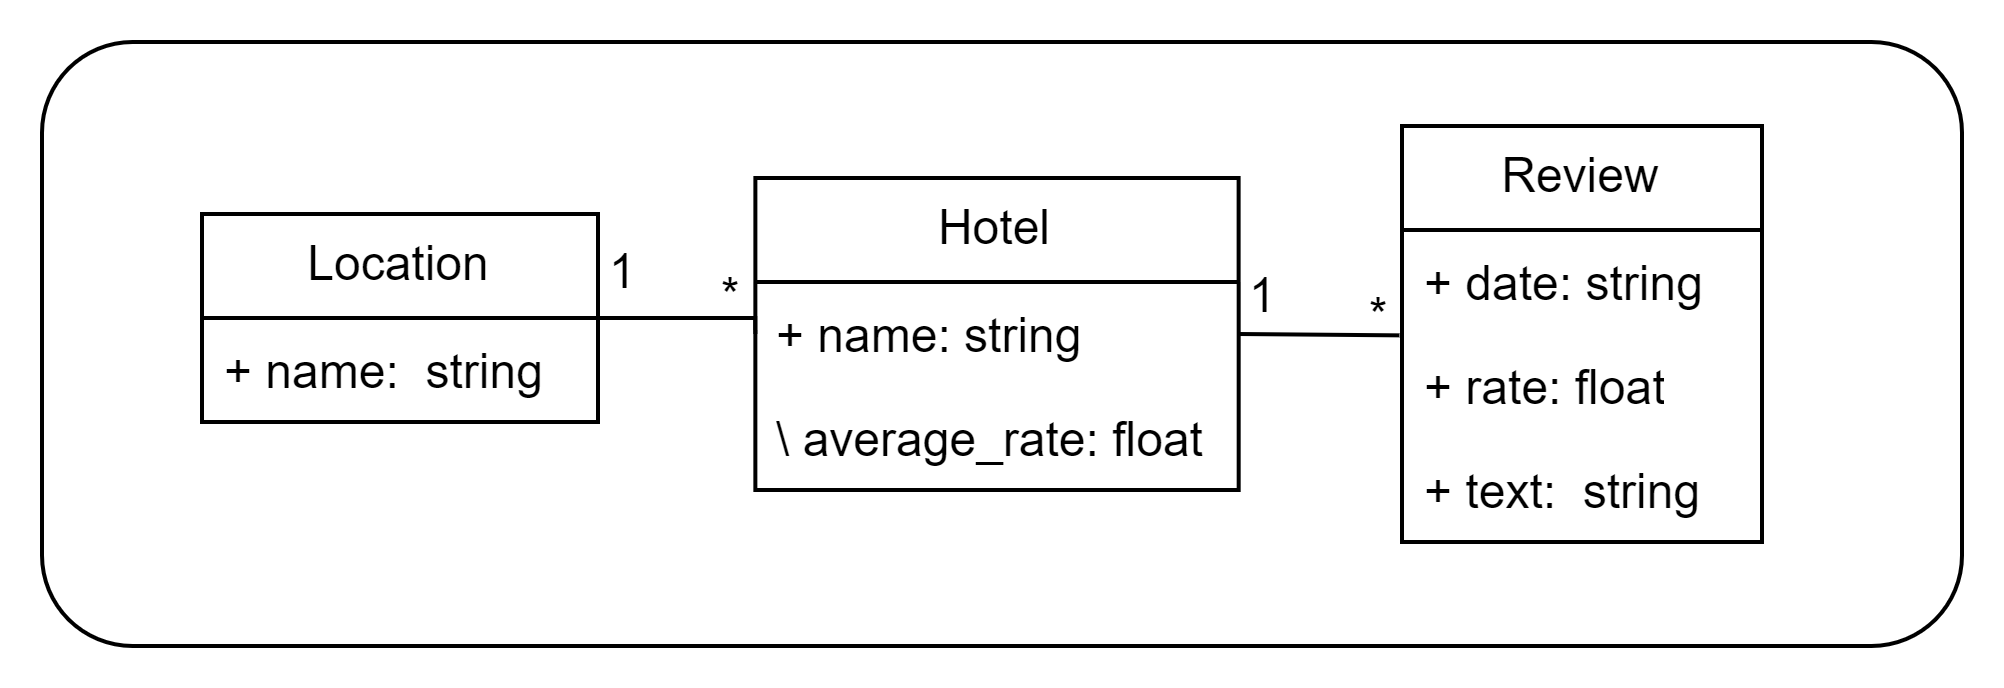
\includegraphics[width=\linewidth]{imgs/UML.png}
  \caption{Data Conceptual Model}
  \Description{TODO}
  \label{fig:uml}
\end{figure}

A hotel is made up of the attributes name, location and average\_rate. Note that average\_rate is a derived attribute that was calculated in the process based on the selected reviews. Each review has the corresponding text, rate and submission date.

Location was also considered a class because, as expected in the hotel scene, there are several hotels per region, mainly in large cities, as shown in figure \ref{fig:hotelLocationDistribution}.

\section{Possible search tasks}

In the course of the data analysis journey, were unveiled valuable insights through the use of a Word Cloud Diagram [Figure \ref{fig:wordcloud}]. This visual representation highlighted the most frequently occurring words in hotel reviews, shedding light on what matters most to travelers. Among these words, some stood out as pivotal in understanding the key factors that influence hotel choice and guest satisfaction.

\textbf{"Location"} emerged as one of the top considerations in travelers' decision-making processes. Whether it's proximity to local attractions, accessibility to transportation hubs, or the overall neighborhood ambiance, the location of a hotel can greatly influence the overall travel experience. Queries like \textbf{"best hotels in [City/Region/Country]"} and \textbf{"hotels near the airport"} can help travelers selecting accommodations that align with their preferred locations and provide convenient access to their destinations.

For many tourists, a good breakfast is an essential element of their stay. The word \textbf{"breakfast"} featured prominently in our Word Cloud [Figure \ref{fig:wordcloud}], suggesting a keen interest in this aspect. Whether it's a hearty breakfast buffet or specialty morning treats, travelers seek accommodations that cater to their breakfast preferences. Queries like \textbf{"Hotels with breakfast/good breakfast"} can assist those who prioritize morning meals.

The words "staff" and "service" were significant contributors. This emphasizes the critical role that hotel staff play in the overall guest experience. From warm welcomes at the reception desk to prompt and efficient room service, exceptional staff service can elevate a stay. Queries such as \textbf{"hotel with a helpful staff"} and \textbf{"affordable room service"} could be instrumental in identifying hotels that excel in providing exceptional service to their guests.

Another one of the foremost considerations in hotel selection is the quality of the room and its amenities. Words like "room," "bed," and "bathroom" featured prominently in our Word Cloud [Figure \ref{fig:wordcloud}], underscoring the importance of these aspects to travelers. Queries related to "room"/"bed" quality or "bathroom" sanitation can guide travelers to accommodations that prioritize comfort and cleanliness.

\section{Conclusions and Future Work}

In conclusion of this milestone, all the planned tasks within the data preparation phase of the project have been successfully completed. This accomplishment marks a crucial turning point in the process of creating a useful hotel search engine that will give tourists useful information and help them make informed choices.

One of the most challenging aspects of the work was developing effective strategies to address the issue of an excessive number of reviews. Substantial effort was invested in determining the best approach to manage and utilize this abundance of information. Through meticulous analysis and innovative methods, a balance was struck between data volume and relevance, ensuring that the dataset remained rich with insights while maintaining a manageable size.

As the project progresses, there are always opportunities for further enhancements and refinements. With the cleansed and consolidated dataset, the next phase of the project will focus on the development of a robust hotel search engine. This engine will allow travelers to explore and filter accommodations according to their preferences, whether related to location, room quality, staff service, or other factors identified during the analysis phase.

%%
%% If your work has an appendix, this is the place to put it.
\appendix

\section{Annexes}

\begin{figure}[H]
  \centering
  \includegraphics[width=\linewidth]{imgs/top_locations.png}
  \caption{Hotel location distribution}
  \Description{TODO}
  \label{fig:hotelLocationDistribution}
\end{figure}

\begin{figure}[H]
  \centering
  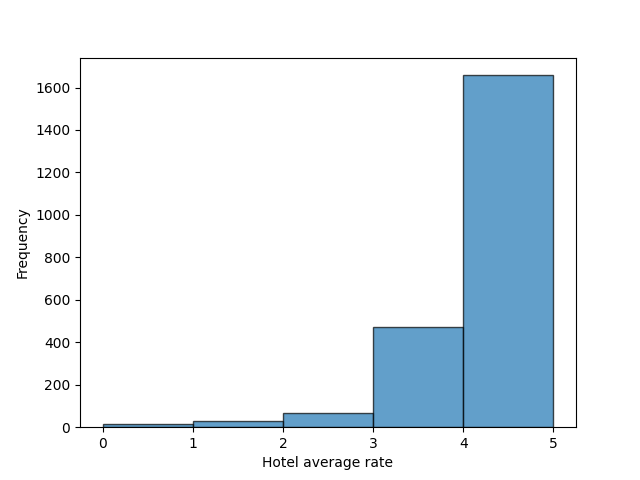
\includegraphics[width=\linewidth]{imgs/rating_distributions.png}
  \caption{Average rate distribution}
  \Description{TODO}
  \label{fig:averageRateDistribution}
\end{figure}

%% Figure 7
\begin{figure}[H]
  \centering
  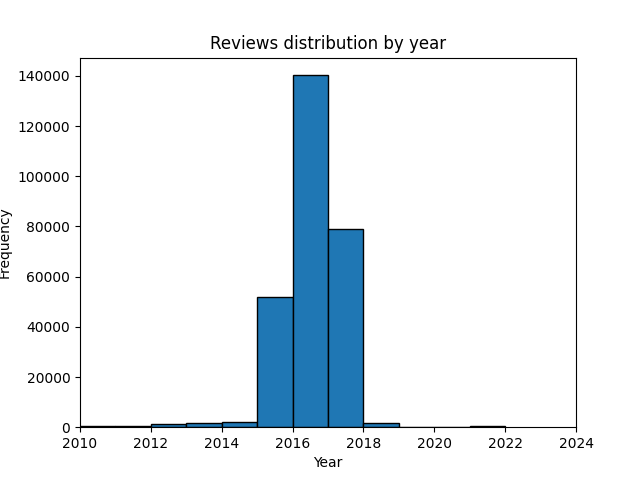
\includegraphics[width=\linewidth]{imgs/date_distributions.png}
  \caption{Reviews distribution per year}
  \Description{TODO}
  \label{fig:reviewsDistributionYear}
\end{figure}

%% Figure 8
\begin{figure}[H]
  \centering
  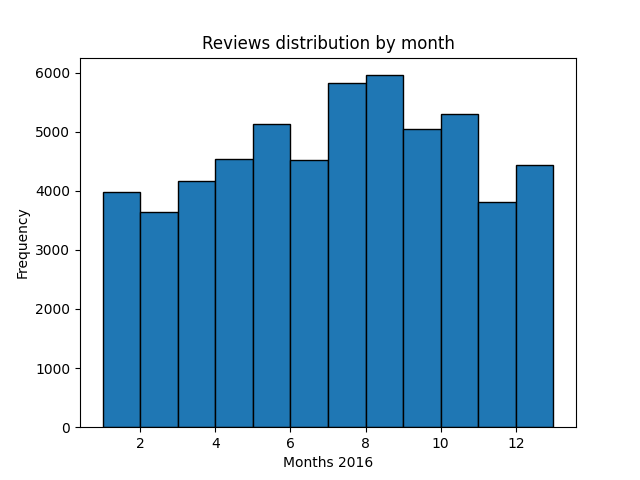
\includegraphics[width=\linewidth]{imgs/date_distributions_2016.png}
  \caption{Month reviews distribution in year 2016}
  \Description{The figure shows a bar chart, the bars represent the frequency (y axis) for every month (x axis of the year), its values range from around 3750 to 6000, the chart shows an increase in frequency in the first nine months (reaching the highest value of around 6000) with exception for the second month (which has the lowest value of the chart with 3750), then there is a decrease in frequency for the last four months with the odd numbered months having slightly higher values than their previous month. }
  \label{fig:monthsDistribution}
\end{figure}

%% Figure 9
\begin{figure}[H]
  \centering
  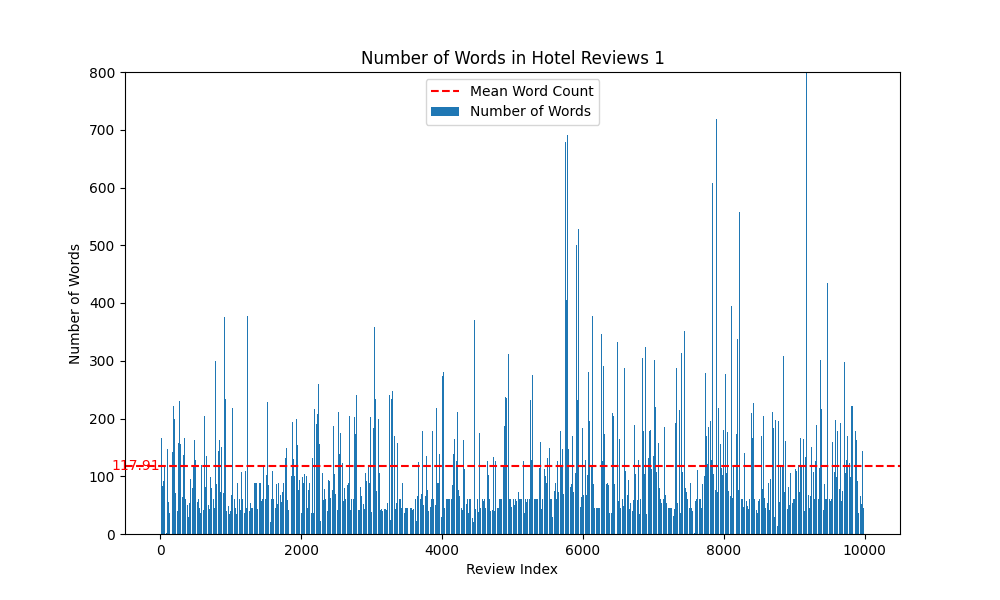
\includegraphics[width=\linewidth]{imgs/word_count_1.png}
  \caption{Average words per review in Datafiniti's Hotel Reviews dataset}
  \label{fig:reviewWords1}
\end{figure}

%% Figure 10
\begin{figure}[H]
  \centering
  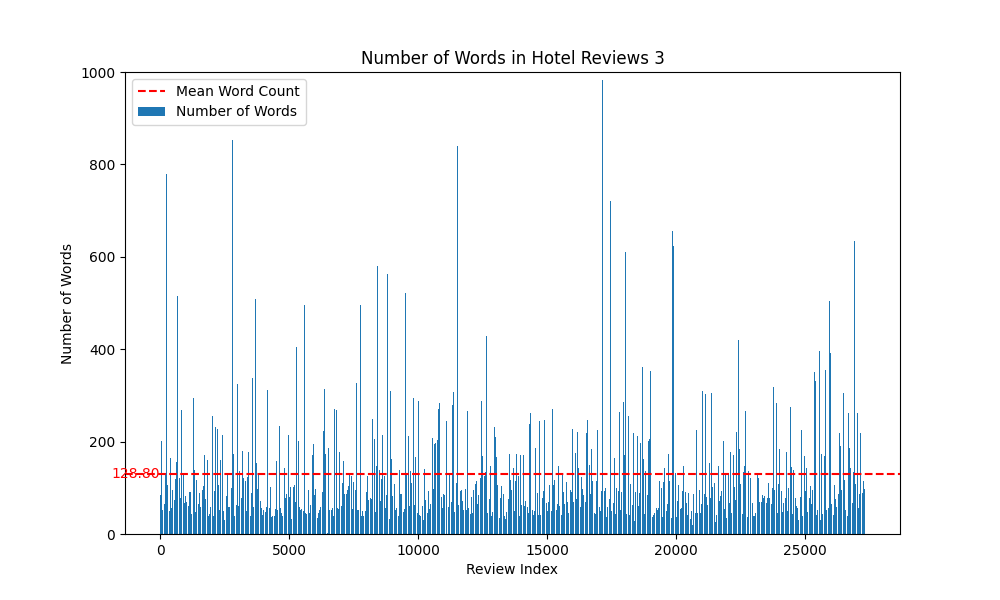
\includegraphics[width=\linewidth]{imgs/word_count_3.png}
  \caption{Average words per review in London Hotel Reviews dataset}
  \label{fig:reviewWords3}
\end{figure}

\nocite{*}
\def\BibTex{BibTeX}
\bibliographystyle{unsrt}
\bibliography{sample-base}

\end{document}
\endinput
%%
%% End of file `sample-sigconf.tex'.
